\section{Durchführung}
\label{sec:Durchführung}
\subsection{Zeitabhängigkeit der Amplitude}
\label{sec:a}
Gemessen wird die Zeitabhängikeit der Amplituden eines gedämpften Schwingkreises, um damit in \ref{sec:Auswertung} den effektiven Dämpfungswiderstand
$R_{eff}$ zu berechnen. Die Messung wird dabei an der in Abbildung \ref{fig:a} dargestellten Schaltung untersucht. 
%Bild einfügen
\begin{figure}[H]
    \centering
    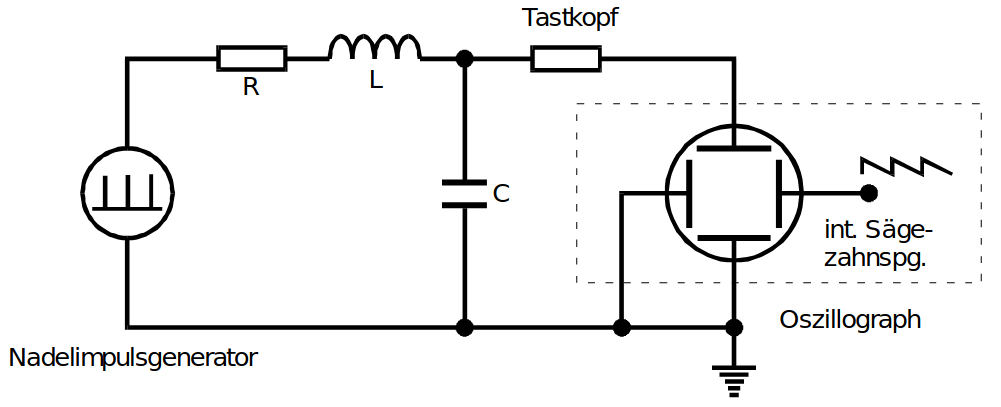
\includegraphics[width=0.6\textwidth]{pictures/Aufbau_a.png}
    \caption{Ein gedämpfter Schwingkreis zur Messung der Zeitabhängigkeit der Amplituden.\cite{AP01}}
    \label{fig:a}
\end{figure}
Dabei wird der Schwingkreis über einen Nadelpulsgenerator so angeregt, dass die Amplitude zwischen den Anregungen um den Faktor drei bis acht 
abgefallen ist. Die Schwingungskurve wird mittels Oszillographen aufgenommen. An dieser werden dann sowohl die zeitlichen Abstände zwischen den Extrema 
der Kurve, als auch die Extremwerte abgelesen und notiert. 
\subsection{Däpfungswiderstand des aperiodischen Grenzfalls}
\label{sec:b}
Zur Bestimmung des Dämpfungswiderstandes, bei dem der aperiodische Grenzfall vorliegt, wird erneut ein Schwingkreis nach Abbildung \ref{fig:a}
verwendet. Nun wird jedoch ein regelbarer Widerstand verbaut. Dieser wird dann von seinem Maximalwert ($\SI{10}{\kilo\ohm}$) langsam verringert. 
Dabei wird die Kurve auf dem Oszillographen beobachtet. Schwingt die Stromstärke in den negativen Bereich über, ist der aperiodische Grenzfall 
nach Kapitel \ref{sec:Fall3} überschritten (vgl. Abbildung\ref{fig:Fall2}). Es wird also jener Wert von dem regelbaren Widerstand abgelesen, bei 
dem die Stromstärke gerade nicht überschwingt. 
\subsection{Frequnzabhängigkeit der Kondensatorspannung}
\label{sec:c}
Um die Frequnzabhängigkeit der Kondensatorspannung zu messen wird ein Versuchsaufbau nach Abbildung \ref{fig:c} benötigt. 
\begin{figure}[H]
    \centering
    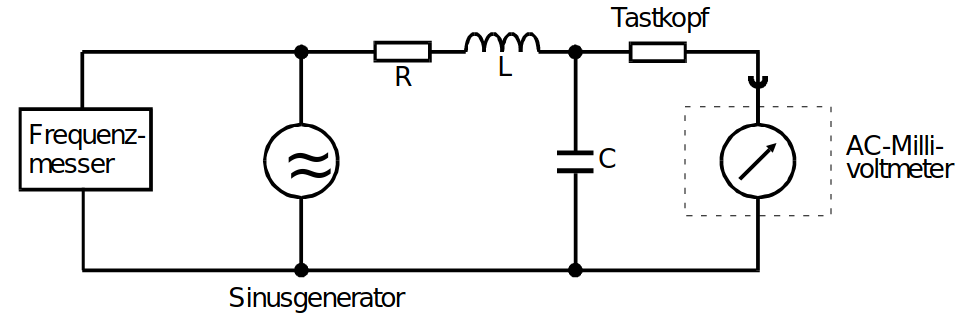
\includegraphics[width=0.6\textwidth]{pictures/Aufbau_b.png}
    \caption{Ein getriebener Schwingkreis zur Messung der Frequenzabhängigkeit der Kondensatorspannung.\cite{AP01}}
    \label{fig:c}
\end{figure}
Der Schwinkreis wird nun über einen Sinusgenerator getrieben. Die Kondensatorspannung $U_C$ wird mittels Voltmeter oder mit einem Oszillographen
aufgenommen. Zusätzlich zu der Kondensatorspannung wird noch die Erregerspannung $U_{err}$ über den Tastkopf in Abhängigkeit von der Frequenz 
gemessen. Auch der Innenwiderstandwiderstand des Sinusgenerators ist zu notieren.